\documentclass{beamer}
\usepackage[english]{babel}
\usepackage[utf8]{inputenc}
\usepackage[T1]{fontenc}
\usepackage{lmodern}
\usepackage{hus-beamer}
\usepackage{ifthen}
\usepackage[bibstyle=authoryear, citestyle=authoryear, maxcitenames=2, maxbibnames=2, backend=bibtex]{biblatex}
%\usepackage[maxbibnames=2]{biblatex}
%citestyle=authoryear or numeric or ...
\addbibresource{ref.bib}

%------ tikZ ------%
\usepackage{tikz}
\usetikzlibrary{tikzmark,overlay-beamer-styles,babel} 
\usetikzlibrary{positioning, arrows}
\usetikzlibrary{backgrounds}
    
\mode<presentation>{
	\usefonttheme{professionalfonts} % normal font for math formulas
	% insert section page with title only
	% before each section
	\AtBeginSection[]{
	\begin{frame}%[noframenumbering] % remove this if you do not want to number section page
	\vfill
	\centering
	\begin{beamercolorbox}[sep=8pt,center,shadow=true,rounded=true]{title}
	\usebeamerfont{title}\insertsectionhead\par%
	\end{beamercolorbox}
	\vfill
	\end{frame}
}
}
%%%%%%%%
%\AtBeginBibliography{\footnotesize} % Footnotesize for Bibliography entries

% \setbeamertemplate{bibliography item}{%
%   \ifboolexpr{ test {\ifentrytype{book}} or test {\ifentrytype{mvbook}}
%     or test {\ifentrytype{collection}} or test {\ifentrytype{mvcollection}}
%     or test {\ifentrytype{reference}} or test {\ifentrytype{mvreference}} }
%     {\setbeamertemplate{bibliography item}[book]}
%     {\ifentrytype{online}
%        {\setbeamertemplate{bibliography item}[online]}
%        {\setbeamertemplate{bibliography item}[article]}}%
%   \usebeamertemplate{bibliography item}}

% \defbibenvironment{bibliography}
%   {\list{}
%      {\settowidth{\labelwidth}{\usebeamertemplate{bibliography item}}%
%       \setlength{\leftmargin}{\labelwidth}%
%       \setlength{\labelsep}{\biblabelsep}%
%       \addtolength{\leftmargin}{\labelsep}%
%       \setlength{\itemsep}{\bibitemsep}%
%       \setlength{\parsep}{\bibparsep}}}
%   {\endlist}
%   {\item}


%\defbibheading{bibliography}[\refname]{}

%------------------%

\begin{document}
\title{Improving Performance}
\subtitle{Week 4}
\author{COMP6252 (Deep Learning Technologies)}
\institute[ECS, University of Southampton]{ECS, University of Southampton} \date{28 April 2022}

\begin{frame}
    \frametitle{Inception (GoogLeNet)}
	\begin{columns}
		
\begin{column}{0.5\textwidth}

    \begin{itemize}
        \item Stack Inception modules on top of each other
        \item Network within a network
    \end{itemize}

    \begin{figure}
        \tikzmarknode{module}{
            \includegraphics[width=1.1\textwidth]{figs/inception.png}
        }
    \end{figure}
		
\end{column}
\begin{column}{0.5\textwidth}
	\vspace{-1.5cm}
	\begin{figure}
        \tikzmarknode{net}{
            \includegraphics[width=0.4\textwidth]{figs/googlenet.png}
        }
    \end{figure}
\end{column}
\end{columns}
\begin{tikzpicture}[overlay,remember picture]
	%\draw [draw=red] (7.5,2.98) rectangle (9.6,4);
	\node (rect) at (8.5,2.73) [draw=red,thick,minimum width=2cm,minimum height=0.8cm] {};
	\draw[-latex,color=red] (rect.west) to (module.east);
	\end{tikzpicture}
\end{frame}

\begin{frame}
	\frametitle{Naive Inception}
\begin{columns}
	\begin{column}{0.5\textwidth}

	\begin{figure}
        \tikzmarknode{naive}{
            \includegraphics[width=1.1\textwidth]{figs/naive_inception.png}
        }
    \end{figure}
\end{column}
\begin{column}{0.5\textwidth}
	\begin{itemize}
		\item Filters applied in parallel
		\item The results are concatenated over the channels
		\item Geometric dimensions of convolutions and maxpooling are the same 
		\item MaxPooling with 3x3 kernel stride=1 and padding=1 to preserve the dimensions
		\item All convolutions are padded so no change in height/width
	\end{itemize}
\end{column}
\end{columns}

\end{frame}

\begin{frame}
	\frametitle{Naive Inception}
\begin{columns}
	\begin{column}{0.5\textwidth}

	
	\begin{figure}
        \tikzmarknode{naive}{
            \includegraphics[width=1.3\textwidth]{figs/naive_inception.png}
        }
    \end{figure}
	\begin{tikzpicture}[overlay,remember picture]
		\node[text=red] (i) at (2.5,1.8){\tiny $28\times 28\times 192$};
		\node[text=red] (a) at (0.8,3.1){\tiny $28\times 28\times 64$};
		\node[text=red] (b) at (2.6,3.1){\tiny $28\times 28\times 128$};
		\node[text=red] (c) at (4.3,3.1){\tiny $28\times 28\times 32$};
		\node[text=red] (d) at (6,3.1){\tiny $28\times 28\times 192$};
		
		\node[text=red] (l1) at (0.8,2.45){\tiny 64 filters};
		\node[text=red] (l2) at (2.45,2.45){\tiny 128 filters};
		\node[text=red] (l3) at (4.2,2.45){\tiny 32 filters};
		\node[text=red] (d) at (2.3,4.5){\tiny $28\times 28\times (64+128+32+192)=28\times 28\times 416$};

		\end{tikzpicture}
\end{column}
\begin{column}{0.5\textwidth}
	\begin{itemize}
		\item Filters applied in parallel
		\item The results are concatenated over the channels
		\item Geometric dimensions of convolutions and maxpooling are the same 
		\item MaxPooling with 3x3 kernel stride=1 and padding=1 to preserve the dimensions
		\item All convolutions are padded so no change in height/width
	\end{itemize}
\end{column}
\end{columns}

\end{frame}

\begin{frame}
	\frametitle{Number of operations}
	We will compute the number of (multiplication ) operations for inception module.
\begin{itemize}
	\item Input is of size HxW
	\item Consider a layer with kernel AxB
	\item all have stride=1 and padding to same 
	\item Therefore each stride performs AxB operations.
	\item Since stride=1 and padding='same' there are HxW strides
	\item Total operations = HxWxAxB 
	\item This is done for each input channel
	\item This is done by every filter so the total number of operations is 
	\item $C_1\times H\times W\times A\times B\times C_2$ 
\end{itemize}
	

\end{frame}


\begin{frame}
	\frametitle{Naive Inception}
\begin{columns}
	\begin{column}{0.5\textwidth}

	
	\begin{figure}
        \tikzmarknode{naive}{
            \includegraphics[width=1.3\textwidth]{figs/naive_inception.png}
        }
    \end{figure}
	\begin{tikzpicture}[overlay,remember picture]
		\node[text=red] (i) at (2.5,1.8){\tiny $28\times 28\times 192$};
		\node[text=red] (a) at (0.8,3.1){\tiny $28\times 28\times 64$};
		\node[text=red] (b) at (2.6,3.1){\tiny $28\times 28\times 128$};
		\node[text=red] (c) at (4.3,3.1){\tiny $28\times 28\times 32$};
		\node[text=red] (d) at (6,3.1){\tiny $28\times 28\times 192$};
		
		\node[text=red] (l1) at (0.8,2.45){\tiny 64 filters};
		\node[text=red] (l2) at (2.45,2.45){\tiny 128 filters};
		\node[text=red] (l3) at (4.2,2.45){\tiny 32 filters};
		\node[text=red] (d) at (2.3,4.5){\tiny $28\times 28\times (64+128+32+192)=28\times 28\times 416$};

		\end{tikzpicture}
\end{column}
\hfill
\begin{column}{0.4\textwidth}
	Multiplication operations
\tiny{
	\begin{itemize}
		\item 1x1: 192x28x28x1x1x64=9633792
		\item 3x3: 192x28x28x3x3x128=173408256
		\item 5x5: 192x28x28x5x5x32=120422400
		\item Total$\approx $ 303M ops
	\end{itemize}
		}
	
\end{column}
\end{columns}

\end{frame}
\begin{frame}
	\frametitle{Naive Inception}
\begin{columns}
	\begin{column}{0.5\textwidth}

	
	\begin{figure}
        \tikzmarknode{naive}{
            \includegraphics[width=1.3\textwidth]{figs/naive_inception.png}
        }
    \end{figure}
	\begin{tikzpicture}[overlay,remember picture]
		\node[text=red] (i) at (2.5,1.8){\tiny $28\times 28\times 192$};
		\node[text=red] (a) at (0.8,3.1){\tiny $28\times 28\times 64$};
		\node[text=red] (b) at (2.6,3.1){\tiny $28\times 28\times 128$};
		\node[text=red] (c) at (4.3,3.1){\tiny $28\times 28\times 32$};
		\node[text=red] (d) at (6,3.1){\tiny $28\times 28\times 192$};
		
		\node[text=red] (l1) at (0.8,2.45){\tiny 64 filters};
		\node[text=red] (l2) at (2.45,2.45){\tiny 128 filters};
		\node[text=red] (l3) at (4.2,2.45){\tiny 32 filters};
		\node[text=red] (d) at (2.3,4.5){\tiny $28\times 28\times (64+128+32+192)=28\times 28\times 416$};

		\end{tikzpicture}
\end{column}
\begin{column}{0.5\textwidth}
	\begin{itemize}
		\item 3x3 conv= (3x3)x(28x28)x(192)x(128)
		\item 5x5 conv= (5x5)x(28x28)x(192)x(132)
		\item total
		\item 173408256 for 3x3
		\item 
	\end{itemize}
\end{column}
\end{columns}

\end{frame}

\begin{frame}
	\frametitle{Inception vs Naive Inception}
\begin{columns}
	\begin{column}{0.5\textwidth}
		\begin{figure}
			\tikzmarknode{naive}{
				\includegraphics[width=1.\textwidth]{figs/naive_inception.png}
			}
		\end{figure}
	\end{column}
	\begin{column}{0.5\textwidth}
		\begin{figure}
			\tikzmarknode{naive}{
				\includegraphics[width=1.\textwidth]{figs/inception.png}
			}
		\end{figure}
	\end{column}
\end{columns}
\end{frame}

\begin{frame}
	\frametitle{Role of 1x1 convolution}
\begin{itemize}
	\item preserves spatial dimensions but reduces depth
\end{itemize}
	

\end{frame}



\begin{frame}
	\frametitle{Naive Inception}
\begin{columns}
	\begin{column}{0.5\textwidth}

	
	\begin{figure}
        \tikzmarknode{naive}{
            \includegraphics[width=1.3\textwidth]{figs/inception.png}
        }
    \end{figure}
	% \begin{tikzpicture}[overlay,remember picture]
	% 	\node[text=red] (i) at (2.5,1.8){\tiny $28\times 28\times 192$};
	% 	\node[text=red] (a) at (0.8,3.1){\tiny $28\times 28\times 64$};
	% 	\node[text=red] (b) at (2.6,3.1){\tiny $28\times 28\times 128$};
	% 	\node[text=red] (c) at (4.3,3.1){\tiny $28\times 28\times 32$};
	% 	\node[text=red] (d) at (6,3.1){\tiny $28\times 28\times 192$};
		
	% 	\node[text=red] (l1) at (0.8,2.45){\tiny 64 filters};
	% 	\node[text=red] (l2) at (2.45,2.45){\tiny 128 filters};
	% 	\node[text=red] (l3) at (4.2,2.45){\tiny 32 filters};
	% 	\node[text=red] (d) at (2.3,4.5){\tiny $28\times 28\times (64+128+32+192)=28\times 28\times 416$};

	% 	\end{tikzpicture}
\end{column}
\hfill
\begin{column}{0.4\textwidth}
	Multiplication operations
\tiny{
	\begin{itemize}
		\item 1x1: 192x28x28x1x1x64=9633792
		\item 3x3: 192x28x28x3x3x128=173408256
		\item 5x5: 192x28x28x5x5x32=120422400
		\item Total$\approx $ 303M ops
	\end{itemize}
		}
	
\end{column}
\end{columns}

\end{frame}
\begin{frame}
	\frametitle{<title>}
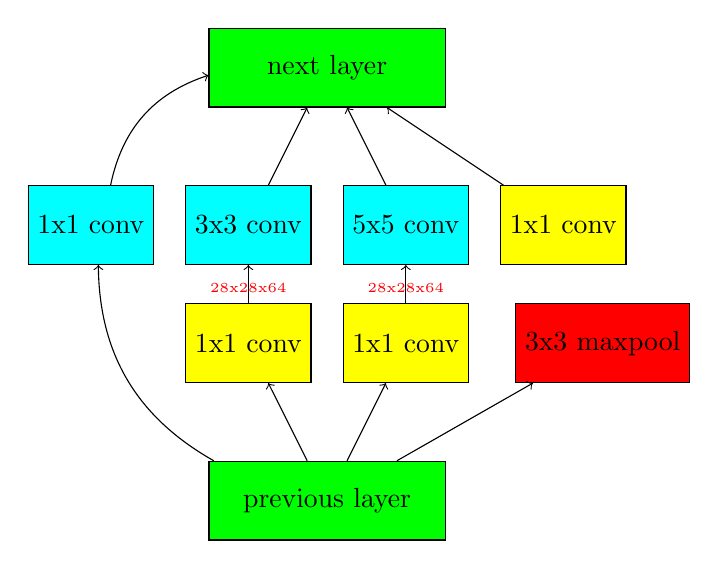
\begin{tikzpicture}
	\node (1x1a) at (0,2) [fill={rgb,1:green,1;blue,1},minimum width=1.5cm,minimum height=1cm,draw] {1x1 conv};
	\node (3x3) at (2,2) [fill={rgb,1:green,1;blue,1},minimum width=1.5cm,minimum height=1cm,draw] {3x3 conv};
	\node (5x5) at (4,2) [fill={rgb,1:green,1;blue,1},minimum width=1.5cm,minimum height=1cm,draw] {5x5 conv};
	\node (1x1b) at (6,2) [fill={rgb,1:red,1;green,1},minimum width=1.5cm,minimum height=1cm,draw] {1x1 conv};
	\node (1x1c) at (4,0.5) [fill={rgb,1:red,1;green,1},minimum width=1.5cm,minimum height=1cm,draw] {1x1 conv};
	\node (1x1d) at (2,0.5) [fill={rgb,1:red,1;green,1},minimum width=1.5cm,minimum height=1cm,draw] {1x1 conv};
	\node (maxpool) at (6.5,0.5) [fill={rgb,1:red,1},minimum width=1.5cm,minimum height=1cm,draw] {3x3 maxpool};

	\node (prev) at (3,-1.5) [fill={green},minimum width=3cm,minimum height=1cm,draw] {previous layer};
	\node (next) at (3,4) [fill={green},minimum width=3cm,minimum height=1cm,draw] {next layer};
	\path[->] (prev) edge [bend left=3em] (1x1a);
	\path[->] (prev) edge  (1x1c);
	\path[->] (prev) edge  (1x1d);
	\path[->] (prev) edge  (maxpool);
	\path[->] (1x1a) edge  [bend left=3em] (next);
	\path[->] (3x3) edge  (next);
	\path[->] (5x5) edge  (next);
	\path[->] (1x1b) edge  (next);
	\path[->] (1x1d) edge  (3x3);
	\path[->] (1x1c) edge  (5x5);
	\node[text=red] at (2,1.2){\tiny 28x28x64};
	\node[text=red] at (4,1.2){\tiny 28x28x64};
\end{tikzpicture}
	

\end{frame}

\end{document}